% ################################
\section{Úvod}

\todo{Zde vysvětlit problémovou situaci a otázky, které se budou v bakalářské/diplomové práci řešit.}

Citace \cite{abadi_tensorflow:_2016, lacey_deep_2016}.


% ################################
\section{Cíl práce}

\todo{Smysl a účel, výzkumné otázky.}


% ################################
\section{Metodika zpracování}

\todo{Cíle, hypotézy/ výzkumné otázky, způsob hledání odpovědí na výzkumné otázky včetně metodiky vlastního výzkumu/šetření, literární rešerše.}


% ################################
\section{Vlastní text práce}

\todo{TODO}

Vlastní řešení dokládá student zpravidla v několika kapitolách. Podle charakteru práce musí student uvážit, zda informace netextové povahy (data, tabulky, obrázky atd.) bude uvádět přímo v textu, nebo je zařadí až za celou práci ve formě příloh, či bude kombinovat oba způsoby. 

Více podrobností viz Metodické pokyny pro vypracování bakalářských a diplomových prací (zveřejňované formou výnosů děkana) a v kurzu MES – Metodologický seminář. 

\subsection{Podkapitola}

Vlastní text práce.

\begin{table}[hbt!]  
\caption{průměry}
\centering
\begin{tabular}{| l | r | r | r | }
\hline
        &        psnr &      ssim &      doba  \\
model &       (db)    &           & gen. (s) \\
\hline
bik. int. & 28.3155 & 0.8566 & 0.0322 \\
nn1000    & 30.1461 & 0.9043 & 0.8109 \\
nn1001    & 30.0324 & 0.9023 & 0.7486 \\
nn1002    & \textbf{30.1886} & \textbf{0.9046} & 1.1731 \\
nn1003    & 30.0390 & 0.9030 & 1.1320 \\
nn1004    & 24.9772 & 0.7172 & 4.4367 \\
nn1005    & 26.1629 & 0.8004 & 4.0475 \\
nn1006    & 27.9129 & 0.8438 & 4.0683 \\
nn1007    & 27.5834 & 0.8360 & 4.2082 \\
\hline
\end{tabular}
\end{table}


\subsubsection{Podřazená kapitola}
Text s odkazem na obrázek \ref{figure:uhk}.


\begin{figure}[hbt!]
 	\begin{center}
    	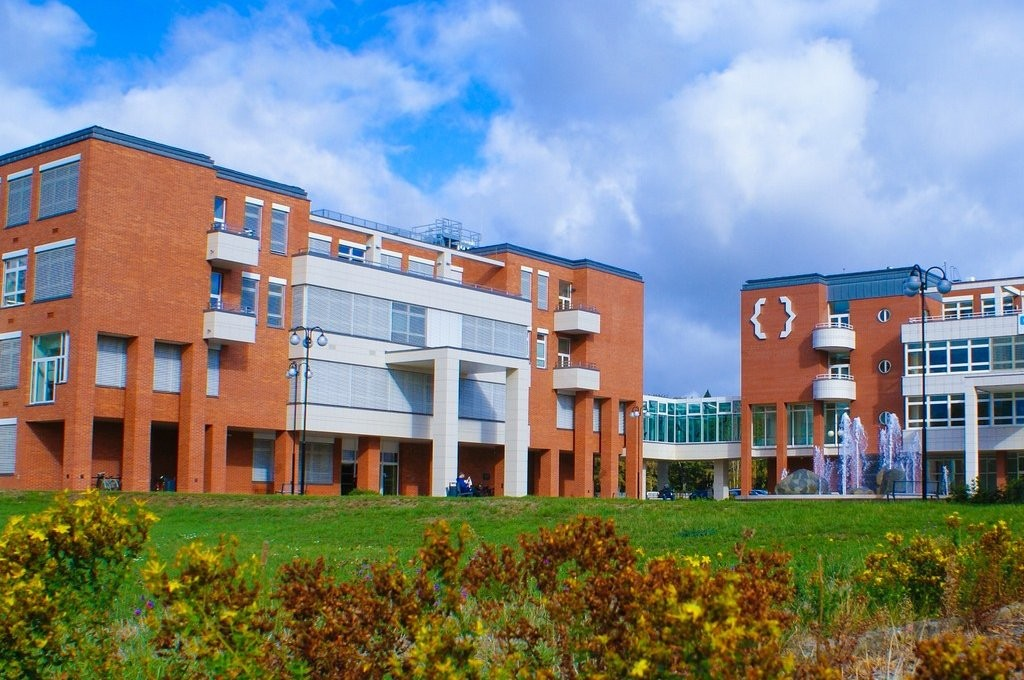
\includegraphics[width=\textwidth]{obrazky/uhk.jpg}
 	\end{center}
 	\caption{Ukázkový obrázek}
	\label{figure:uhk}
\end{figure} 


% ################################
\section{Souhrn výsledků}

\todo{Souhrn vlastních výsledků získaných v průběhu řešení problému.}

\noindent\todo{Zkratka} \Ac{DNN}


% ################################
\section{Závěry a doporučení}

\todo{Kritická diskuze nad výsledky, ke kterým autor dospěl (soulad výsledků  literaturou či předpoklady; výsledky a okolnosti, které zvláště ovlivnily předkládanou práci atd.). Je vhodné naznačit i případné další (popř. alternativní) možnosti zkoumání dané problematiky a otevřené problémy pro další studium. }
